%KELOMPOK 2 Pemasukan
%\begin{itemize}
%\item Imron Sumadireja (1164076)
%\item Jesron Marudut Hatuan (1164077)
%\item Lusia Violita Aprilian (1164080)
%\item Mhd. Zulfikar Akram Nst. (1164081)
%\end{itemize}

\section{Pengertian HTTP}
Protokol HTTP atau Hypertext Transfer Protocol merupakan sebuah protokol untuk meminta dan menjawab antara client dengan server. HTTP juga merupakan protokol jaringan lapisan aplikasi yang digunakan untuk sistem informasi terdistribusi, kolaboratif, dan menggunakan hypermedia. Misalnya pada aplikasi mobile dan Dropbox Service HTTP digunakan  sebagai protokol yang dapat mendistribusikan animasi gambar dan suara yang bersumber dari Dropbox Service\cite{herdiansyah2013pembangunan}.

\subsection{HTTP Protokol Untuk Streaming}
HTTP protokol digunakan dalam streaming karena protokol ini sangat mudah untuk diakses dimanapun. HTTP protokol ini menyediakan movie dari standart web server dengan nama lain `pseudo streaming' atau `progressive download' dikenal juga dengan fast start. Pada saat kita mendownload sebuah video dan filenya sudah di download tetapi bisa di play pada saat sebelum download selesai. Terlihat seperti true streaming. HTTP bisa memiliki data rate yang lebih tinggi, sehingga bisa memiliki kualitas yang lebih tinggi, bahkan untuk file yang telah di download bisa di play berulang - ulang. HTTP juga bisa untuk streaming semua jenis data quicktime\cite{putra2010analisis}.

\subsection{Kemampuan protokol HTTP}
Sebagai sebuah protokol jaringan aplikasi yang digunakan untuk sistem informasi terdistribusi, Hypertext Transfer Protokol (HTTP) mempunyai kemampuan sebagai berikut ini;
1. Hypertext Transfer Protokol (HTTP) mampu mengirim tipe data yang komplit sama halnya dengan satu pesan yang memakai satu format untuk MIME mail internet. Sebab itu sebuah Website dapat melebihi hypertext ke hypertmedia dan website server dapat melayani client dengan informasi informasi yang berupa teks, suara, video dan grafik yang diintergrasikan menggunakan dokumen HTML.
2. Hypertext Transfer Protocol dapat memfasilitasi komunikasi antar protokol lain yang mengunakan gateway yang berbeda dengan client HTTP. Dari skema penamaan URL mengidentifikasikan bahwa tidak lokasi saja tetapi protokol yang dibutuhkan untuk menerima sumber dayanya\cite{lusiana2009sistem}.

\subsection{cara menggunakan HTTP melalui TLS}
Secara konseptual, HTTP / TLS sangat sederhana, Cukup gunakan HTTP melalui TLS seperti menggunakan HTTP melalui TCP. Agen yang bertindak sebagai klien HTTP yang juga harus bertindak sebagai klien TLS. Hal ini harus terkoneksi ke server pada port yang sesuai dan kemudian mengirim Klien TLS. Ketika hubungan TLS telah selesai. Klien kemudian dapat memulai permintaan HTTP pertama. Semua data HTTP harus dikirim sebagai `data aplikasi' TLS. HTTP berjalan normal, termasuk koneksi yang dipertahankan, harus diikuti\cite{rescorla2000http}.

\section{HTTP versi 2}
HTTP versi 2 adalah versi berikutnya dari HTTP dan didasarkan pada Google SPDY, yang dirancang untuk mempercepat loading halaman web dan pengalaman browsing. HTTP versi 2 adalah standar baru dan akan mengambil alih protokol HTTP yang saat ini digunakan oleh sebagian besar situs di internet. HTTP versi 2 ini merupakan protokol yang lebih modern, dimana http versi 2 dapat meningkatkan kecepatan browsing web dengan menggunakan cara-cara terbaru. HTTP versi 2 lebih cepat dari HTTP dalam hal transfer rate, hal ini dipengarui oleh salah satunya, yaitu server push. Adanya server push membantu mengurangi waktu tunggu yang dialami oleh browser\cite{engku2016analisis}.

\subsection{Tujuan HTTP versi 2}
HTTP versi 2 merupakan sebuah protokol web versi terbaru yang baru saja diresmikan standarnya oleh IETF. Tujuan utamanya dibuat HTTP versi 2 adalah untuk memperbaiki kelemahan yang ada pada HTTP versi 1.1 salah satu kelemahannya yakni ketika browser meminta halaman, server akan mengirimkan dokumen HTML, kemudian perlu menunggu browser untuk mengurai dokumen HTML untuk memunculkan request untuk semua aset yang tertanam, sebelum server dapat mengirim JavaScript, gambar dan CSS. Teknologi server push pada HTTP versi 2 memungkinkan server untuk menghindari perputaran ini dengan cara `mendorong' aset-aset baru dari server ke klien\cite{engku2016analisis}.

\section{Sistem Komunikasi Langsung Multimedia Yang Terhubung Dengan HTTP Protocol}
Sistem komunikasi langsung multimedia yang terhubung dengan Protokol HTTP terdiri dari program aplikasi dan Server Web, di mana program aplikasi diinstal menjadi sejumlah komputer pribadi klien (PC), berada di dalamnya PC sedemikian rupa sehingga mereka ditampilkan selama berjam-jam di PCS menempati sebagian Ruang pada tampilan PC, dan terhubung setiap saat dengan server Web melalui HTTP; Web server memiliki antarmuka CGI dan terhubung ke masing-masing PCS melalui sirkuit komunikasi untuk mengeksekusi Program dan aplikasi komunikasi HTTP, dan masing-masing klien dapat mentransfer (chat) surat elektronik dengan satu sama lain pseudo-real time Via Internet dan / atau Intranet menggunakan program aplikasi\cite{nishizawa2005multimedia}.

\section{Versi HTTP}
Dalam skema penomoran, HTTP menggunakan skema `<Major>.<Minor>' untuk menunjukkan versi versi dari setiap prtotokol. Kebijakan dibuatnya versi protokol untuk memungkinkan pengirim untuk memilih format pesan dan kapasitas dalam memahami setiap komunikasi HTTP lebih lanjut, dari pada fitur-fitur yang diperoleh melalui komunikasi. Dan tidak hanya perbedaan yang dibuat ke nomor untuk setiap versi agar penambahan komponen-komponen pesan yang tidak mempengaruhi sifat dari komunikasi tersebut\cite{berners1996hypertext}.

\subsection{Versi HTTP #2}
Angka <minor> meningkat ketika terjadi perubahan saat protokol menambahkan fitur yang tidak mengubah algortima pesan, akan tetapi menambah makna pesan dan menyiratkan kemampuan pengirim tambahan. Angka <major> meningkat saat protokol dalam pesan telah diubah. Versi HTTP ditunjukan oleh bidang versi HTTP pada baris pertama pesan. Apabila versi protokol tidak ditentukan, penerima harus menggangap bahwa pesan tersebut dalam format HTTP/0,9 yang sederhana. HTTP-version = `HTTP' `/' 1*DIGIT `.' 1*DIGIT. Perlu diperhatikan bahwa nomor besar dan kecil harus diperlakukan sebagai bilangan bulat terpisah dan masing-masing dapat meningkat lebih tinggi dari satu digit. Dengan begitu, HTTP/2.4 merupakan versi HTTP terendah dari HTTP/2.13. Memimpin 0 harus diabaikan oleh penerima dan tidak akan pernah dihasilkan oleh pengirim\cite{berner1996hypertext}.

\subsection{Versi HTTP #3}
Dokumen ini yang membedakan kedua versi 0.9 dan 1.0 dari HTTP. Aplikasi mengirim pesan Full-Request atau Full-Response, sebagaimana didefinisikan oleh spesifikasi ini, harus menyertakan versi HTTP `HTTP/1.0'.
Server HTTP/1.0 harus:
\begin{itemsize}
	\item Mengetahui format Permintaan-Baris untuk meminta HTTP/0.9 dan HTTP/1.0;
	\item Paham kepada permintaan yang valid dalam format HTTP/0.9 atau HTTP/1.0;
	\item Respon secara tepat dengan pesan dalam versi protokol yang sama dengan klien.
	\end{itemsize}
Klien HTTP/1.0 harus;
\begin{itemsize}Kenal format Status-Line untuk menanggapi HTTP/1.0;
	\item Memahami respons valid baik dalam format HTTP/0.9 atau HTTP/1.0
	\Item Proxy dan gateway harus teliti dalam meneruskan permintaan yang diterima dalam format yang berbeda dari HTTP yang asli. Karena setiap versi protokol punya kemampuan mengirim protokol, proxy atau gateway tidak bisa mengirim pesan dengan versi yang lebih besar dari versi asli; apabila permintaan versi yang lebih tinggi diterima, maka proxy atau gateway harus lebih dahulu menurunkan tingkatan versi dari format asli agar dapat diteruskan; proxy/gateway dapat diteruskan apabila mengikuti syarat-syarat server yang tadi\end{itemsize}\cite{berner1996hypertext}. 

 
\section{HTTP Message}
Http Messages adalah rangkaian blok data yang dikirim antar aplikasi HTTP. Blok data diawali dengan teks yang berisi meta information. Teks ini menggambarkan konten pesan dari HTTP message. Setiap HTTP message berisi tentang request dari client atau response dari server. HTTP message terbagi menjadi 3 bagian, yaitu: start line, headers, dan body\cite{hartono2013desain}.

\subsection{3 Bagian HTTP Message}
Start Line merupakan bagian pertama dari HTTP message yang memberikan gambaran data yang dikirim. Header merupakan bagian HTTPmessage yang berfungsi untuk memberikan informasi atribut data. Sedangkan bagian Body merupakan bagian HTTP message yang berisi pesan yang inign dikirim. Pada penggunaannya terdapat perbedaan formmat penulisan HTTP message yang dikirimkan dari client ke server (http request) dengan HTTP message yang dikirimkan dari server ke client (http response)\cite{hartono2013desain}.

\section{Kompatibilitas HTTP dengan Proxy, Firewalls, dan NAT}
Salah satu alasan mengapa penggunaan HTTP adalah kemampuannya untuk lulus melalui proksi, firewall, atau penerjemah alamat jaringan (NAT). Satu konsekuensi yang tidak menguntungkan dari firewall dan NAT adalah yang mereka dibuat lebih sulit untuk menyebarkan aplikasi Internet baru, dengan meminta eksplisit izin (atau bahkan peningkatan perangkat lunak firewall atau NAT) pada akomodasi setiap protokol baru. Keberadaan firewall dan NAT menciptakan insentif yang kuat untuk perancang protokol untuk lapisan baru aplikasi di atas protokol yang ada, termasuk HTTP. Namun, jika firewall situs mencegah penggunaan protokol yang tidak dikenal, ini agaknya merupakan keputusan kebijakan yang sadar dari pihak administrator firewall. Sementara itu dapat diperdebatkan bahwa kebijakan tersebut nilai terbatas dalam meningkatkan keamanan, di samping itu nomor port terkenal sangat berguna untuk berbagai tujuan, dan kelebihan nomor port mengikis utilitas ini. Mencoba untuk menghindari kebijakan keamanan situs tidak dapat diterima pembenaran untuk melakukannya. Akan berguna untuk menetapkan pedoman untuk `firewall-friendly' protokol, untuk memudahkan firewall yang ada agar kompatibel dengan protokol baru
\cite{moore2002use}.

\section{Konsep Web Client dan Web Server}

\begin{figure}[ht]
\centerline{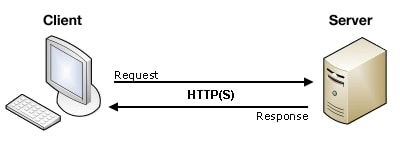
\includegraphics[width=1\textwidth]{figures/2http.jpg}}
\caption{Client Server}
\label{2http}
\end{figure}

Pada gambar \ref{2http} dijelaskan bahwa setiap web content berada pada web server. Web server berkomunikasi menggunakan HTTP sebagai protokol, maka sering disebut sebagai HTTP server. Proses pengiriman data dimulai dari HTTP client yang mengirimkan HTTP request ke server. HTTP request tersebut akan diterima dan diolah oleh server, kemudian server akan mengirimkan kembali HTTP response pada client. HTTP client dan HTTP server merupakan komponen yang membentuk World Wide Web (WWW).

\section{Blok bangunan Web Service}

Gambar \ref{2webservicehttp} merupakan blok bangunan web service yang menyediakan fasilitas komunikasi jarak jauh antara dua aplikasi yang merupakan layer arsitektur web service, berikut penjelasannya:
\begin{itemize}
\item Layer 1 : protokol internet standar yang digunakan sebagai sarana transportasi yakni HTTP dan TCP/IP.
\item Layer 2 : Simple Object Access Protocol (SOAP) yang berbasiskan XML dan digunakan untuk pertukaran informasi antar sekelompok layanan.
\item Layer 3 : Web Service Definition Language (WSDL) digunakan untuk mendeskripsikan attribute layanan.
\item Layer 4 : Universal Description, Discovery and Integration, yang mana merupakan direktori pusat untuk deskripsi suatu layanan\cite{deviana2013penerapan}.
\end{itemize}

\begin{figure}[ht]
\centerline{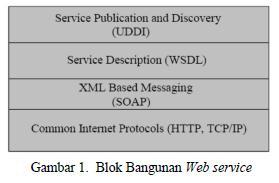
\includegraphics[width=1\textwidth]{figures/2webservicehttp.jpg}}
\caption{Blok bangunan web service}
\label{2webservicehttp}
\end{figure}

\section{HTTP Bit Rate}
Versi streaming bit rate adaptif digunakan oleh Adobe Sistem, Apple, Microsoft, dan Octoshape. Kedua Adobe Flash Player dan Flash Media Server mendukung bit-rate adaptif streaming melalui protokol RTMP tradisional, serta HTTP mirip dengan solusi berbasis HTTP dari Apple dan Microsoft. Streaming berbasis HTTP memiliki keuntungan tidak membutuhkan port firewall dibuka di luar normal port yang digunakan oleh browser web. Streaming berbasis HTTP juga memungkinkan fragmen video di-cache oleh browser, proksi, dan CDN. Implementasi Apple dari streaming HTTP, Http Live Streaming (HLS) disediakan sebagai bagian dari Quick-Time mereka X, dan sistem perangkat lunak iPhone. Apple baru saja merilis iPad juga menggunakan HLS. HLS bekerja dengan memecah aliran menjadi beberapa unduhan file berbasis HTTP kecil yang dimuat di tingkat adaptif variabel. HTTP bit rate streaming adaptif adalah berdasarkan unduhan progresif HTTP, tetapi bertentangan dengan pendekatan sebelumnya, di sini file sangat kecil, sehingga mereka dapat dibandingkan dengan streaming paket, seperti halnya kasus menggunakan RTSP dan RTP
\cite{hsu2013startup}.

\section{HTTP Sniffer}
HTTP Sniffer adalah sebuah protokol analyzer dan alat reassembly dengan platform yang hanya dapat digunakan di windows. HTTP Sniffer ini dapat menangkap paket IP yang berisi pesan HTTP, membangun kembali sesi HTTP, dan reassemles file yang dikirim melalui protokol HTTP. HTTP Sniffer merupakan protokol yang menyediakan analisis yang nyata dari setiap konten ketika sedang menangkap sebuah paket, meanalisis, parsing dan pesan decoding HTTP\cite{sujana2015perangkat}.

\subsection{Fitur HTTP Sniffer}
HTTP Sniffer memiliki beberapa fitur yang mengakui aliran direkonstruksi setiap sesi TCP. HTTP Sniffer juga mendukung HTML, XML, GIF, JPG dan juga jenis file lainnya. Selain itu HTTP Sniffer juga menyediakan mekanisme fleksibel untuk memantau target khusus host dan jenis  file. HTTP Sniffer juga menyesuaikan ekspor log file dalam format HTML atu CSV.  Berikut ini adalah beberapa fitur dari HTTP Sniffer :
\begin{itemize}
\item Powerfull berkas HTTP Rebuilder
\item Beberapa jenis berkas dukungan
\item Powerfull packet untuk menangkap filter
\item Logging yang disesuaikan\cite{sujana2015perangkat}.
\end{itemize}

\section{Proxy HTTP}
Proxy http mampu menangani lalu lintas pada URL yang diawali dengan shttp: // atau http:// serta cenderung murah dan efektif dalam menyembunyikan alamat IP. HTTP merupakan protokol request/response antara client dan server. Client membuat sebuah HTTP request, seperti web browser. Server – merupakan komputer yang menyimpan atau membuat file HTML. Sebuah client HTTP akan menginisialisasi sebuah request dengan membangun sebuah koneksi TCP ke port 80 (default) , Sebuah Server HTTP akan mendengarkan port. Saat menerima request, server akan mengirimkan kembali status seperti : `(HTTP/1.1 200) OK', dan sebuah message untuk dirinya sendiri\cite{farhanah2011pengembangan}.

\section{Protokol Jaringan OSI Layer}
Model OSI menerapkan konsep yang dikenal dengan enkapsulasi. Enkapsulasi itu sendiri merupakan proses atau metode membungkus data dari satu lapisan model OSI dalam struktur data baru ke lapisan model OSI yang lainnya. Berikut merupakan lapisan-lapisan yang terdapat pada model OSI:
\begin{itemize}
\item Physical Layer
\item Data Link Layer
\item Network Layer
\item Transport Layer
\item Session Layer
\item Presentasi Layer
\item Application Layer
\end{itemize}
Pada layer Application, terdiri dari beberapa protokol yang digunakan salah satunya yakni HTTP (Hypertext Transfer Protocol) Protokol yang dipergunakan untuk mentransfer dokumen dan web dalam sebuah web browser, yang biasa digunakan melalui www. HTTP juga merupakan protokol yang meminta sekaligus menjawab antara klien dan server\cite{sujana2015perangkat}.

\section{Method HTTP/1.0}
\begin{itemsize}
\item GET
Metode GET untuk mengambil informasi-informasi apa pun yang diidentifikasi oleh Request-URI. Apabila Request-URI mengacu pada proses produksi data, maka data yang dihasilkan adakn dikemabalikan sebagai etentitas dalam respon dan bukan dari sumber text dari proses tersebut, kecuali teks itu kebetulan jadi output dari prosesnya.

\item HEAD
Metode Head identik dengan Metode Get, terkecuali server tidak warus mengembalikan Badan Entitas dalam respon apapun. Metainformasi yang terkandung dalam head HTTP sebagai respon atas permintaan HEAD yang identtik dengan informasi yang dikirim sebagai tanggapan atas permintaan GET. Metode ini bisa digunakan untuk mengambil informasi tentang sumber daya yang diidentifikasi oleh Request-URI tanpa mentransfer Badan Entitas sendiri.

\item POST
Metode POST biasanya dipakai untuk meminta server tujuan  agar menerima entitas yang terlampir dalam permintaan baru dari Request-URI di Permintaan-Baris. Post dirancang untuk memungkinkan metode yang seragam untuk mencakup fungsi berikut;
\begin{itemsize}
	\item Anotasi sumber daya yang ada;
	\item Memposting pesan ke buletin, newsgroup, atau kelompok artikel serupa;
	\item Menyediakan blok data, seperti hasil mengirimkan formulir ke proses penanganan data;
	\item Memperluas databse melalui operasi tambahan.
	\end{itemsize}
\end{itemsize}\cite{berner1996hypertext}.